\documentclass[serif]{beamer}

% ---------------------------------------------------------

\usepackage[utf8]{inputenc}
\usepackage[T1]{fontenc}
\usepackage[english]{babel}

% ---------------------------------------------------------

\usepackage{appendixnumberbeamer}

\setbeamertemplate{navigation symbols}{}

\addtobeamertemplate{footline}{%
	\hspace*{\fill}%
	\llap{%
		\insertframenumber\,/\,\inserttotalframenumber%
		\hspace{5pt}%
	}
	\vskip4pt%
}

% ---------------------------------------------------------

\usepackage{changepage}

\usepackage{tikz}

% ---------------------------------------------------------

\usepackage{amsmath}

\usepackage{mathtools}

\usepackage{mathpartir}
\let\TirName\textsc
\renewcommand{\DefTirName}[1]{\hypertarget{#1}{\TirName {#1}}}
\newcommand{\RefTirName}[1]{\hyperlink{#1}{\TirName {#1}}}

\let\oldexists\exists
\let\exists\relax\DeclareMathOperator{\exists}{\oldexists}
\let\oldforall\forall
\let\forall\relax\DeclareMathOperator{\forall}{\oldforall}

\DeclareMathOperator{\lambdaAbs}{\lambda}
\DeclareMathOperator{\muAbs}{\mu}
\DeclareMathOperator{\nuAbs}{\nu}

% ---------------------------------------------------------

\usepackage{overtools}

\usepackage{macros}

\usepackage{mylistings}

% ---------------------------------------------------------

\title{
	Verifying Tail Modulo Cons using \\ Relational Separation Logic
}
\author{
	\underline{Clément Allain} \\
	Gabriel Scherer \\
	François Pottier
}
\institute{
	INRIA Paris
}

% ---------------------------------------------------------
% ---------------------------------------------------------

\begin{document}

% ---------------------------------------------------------

\begin{frame}
\titlepage
\end{frame}

% ---------------------------------------------------------

\begin{frame}
\centering
\Large
\textcolor{beamer@blendedblue}{\hl<2>{Verifying} \hl<1>{Tail Modulo Cons} using \\ \hl<3>{Relational Separation Logic}}
\vfill
\only<1>{
    Program transformation implemented in the \OCaml compiler by Frédéric Bour, Basile Clément \& Gabriel Scherer.
}
\only<2>{
    Formalize the transformation and its soundness.
}
\only<3>{
    Prove soundness using an adequate \Iris binary logical relation à la \Simuliris.
}
\end{frame}
\begin{frame}[fragile]{The \texttt{map} problem: natural implementation}
\begin{adjustwidth}{-1.2em}{-1.2em}
\begin{lstlisting}
let rec %\textcolor{red}{map}% f xs =
  match xs with
  | [] ->
      []
  | x :: xs ->
      let y = f x in
      %\textcolor{teal}{y ::}% %\textcolor{red}{map}% f xs
\end{lstlisting}
\vfill
\begin{lstlisting}
# List.init 250_000 (fun _ -> ())
  |> map Fun.id
  |> ignore
  ;;
Stack overflow during evaluation (looping recursion?).
\end{lstlisting}
\end{adjustwidth}
\end{frame}

\begin{frame}{The \texttt{map} problem: natural implementation}
\centering
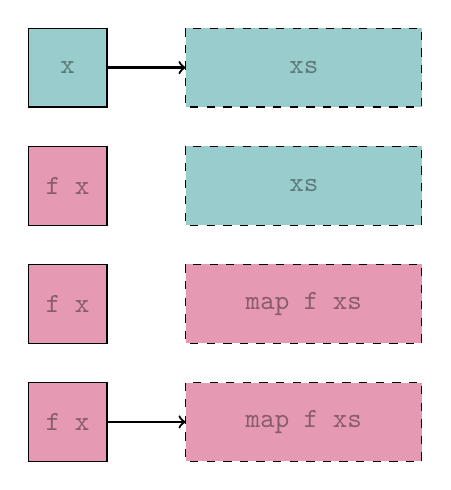
\begin{tikzpicture}[yscale=-1]
    \draw [fill=teal, fill opacity=0.4] (0,0) rectangle (1,1) node [pos=.5] {\texttt{x}} ;
    \draw [fill=teal, fill opacity=0.4, dashed] (2,0) rectangle (5,1) node [pos=.5] {\texttt{xs}} ;
    \draw [thick, ->] (1,0.5) -- (2,0.5) ;
    
    \draw [fill=purple, fill opacity=0.4] (0,1.5) rectangle (1,2.5) node [pos=.5] {\texttt{f x}} ;
    \draw [fill=teal, fill opacity=0.4, dashed] (2,1.5) rectangle (5,2.5) node [pos=.5] {\texttt{xs}} ;
    
    \draw [fill=purple, fill opacity=0.4] (0,3) rectangle (1,4) node [pos=.5] {\texttt{f x}} ;
    \draw [fill=purple, fill opacity=0.4, dashed] (2,3) rectangle (5,4) node [pos=.5] {\texttt{map f xs}} ;
    
    \draw [fill=purple, fill opacity=0.4] (0,4.5) rectangle (1,5.5) node [pos=.5] {\texttt{f x}} ;
    \draw [fill=purple, fill opacity=0.4, dashed] (2,4.5) rectangle (5,5.5) node [pos=.5] {\texttt{map f xs}} ;
    \draw [thick, ->] (1,5) -- (2,5) ;
\end{tikzpicture}
\end{frame}

\begin{frame}[fragile]{The \texttt{map} problem: APS implementation}
\begin{lstlisting}
let rec %\textcolor{red}{map}% %\textcolor{teal}{ys}% f xs =
  match xs with
  | [] ->
      List.rev ys
  | x :: xs ->
      let y = f x in
      %\textcolor{red}{map}% %\textcolor{teal}{(y ::\ ys)}% f xs
let map xs =
  map [] f xs
\end{lstlisting}
\vfill
\begin{lstlisting}
# List.init 250_000 (fun _ -> ())
  |> map Fun.id
  |> ignore
  ;;
- : unit = ()
\end{lstlisting}
\end{frame}

\begin{frame}{The \texttt{map} problem: APS implementation}
\centering
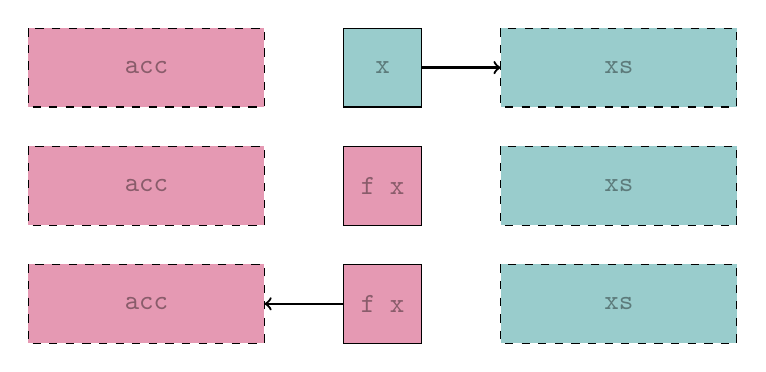
\begin{tikzpicture}[yscale=-1]
    \draw [fill=purple, fill opacity=0.4, dashed] (0,0) rectangle (3,1) node [pos=.5] {\texttt{acc}} ;
    \draw [fill=teal, fill opacity=0.4] (4,0) rectangle (5,1) node [pos=.5] {\texttt{x}} ;
    \draw [fill=teal, fill opacity=0.4, dashed] (6,0) rectangle (9,1) node [pos=.5] {\texttt{xs}} ;
    \draw [thick, ->] (5,0.5) -- (6,0.5) ;
    
    \draw [fill=purple, fill opacity=0.4, dashed] (0,1.5) rectangle (3,2.5) node [pos=.5] {\texttt{acc}} ;
    \draw [fill=purple, fill opacity=0.4] (4,1.5) rectangle (5,2.5) node [pos=.5] {\texttt{f x}} ;
    \draw [fill=teal, fill opacity=0.4, dashed] (6,1.5) rectangle (9,2.5) node [pos=.5] {\texttt{xs}} ;
    
    \draw [fill=purple, fill opacity=0.4, dashed] (0,3) rectangle (3,4) node [pos=.5] {\texttt{acc}} ;
    \draw [fill=purple, fill opacity=0.4] (4,3) rectangle (5,4) node [pos=.5] {\texttt{f x}} ;
    \draw [fill=teal, fill opacity=0.4, dashed] (6,3) rectangle (9,4) node [pos=.5] {\texttt{xs}} ;
    \draw [thick, ->] (4,3.5) -- (3,3.5) ;
\end{tikzpicture}
\end{frame}

\begin{frame}{The \texttt{map} problem: DPS implementation}
\centering
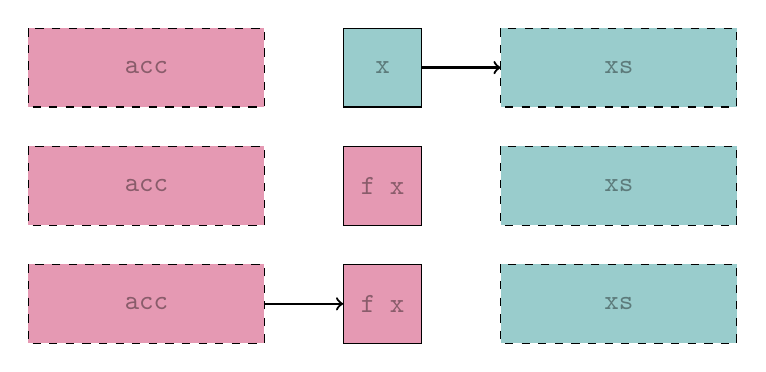
\begin{tikzpicture}[yscale=-1]
    \draw [fill=purple, fill opacity=0.4, dashed] (0,0) rectangle (3,1) node [pos=.5] {\texttt{acc}} ;
    \draw [fill=teal, fill opacity=0.4] (4,0) rectangle (5,1) node [pos=.5] {\texttt{x}} ;
    \draw [fill=teal, fill opacity=0.4, dashed] (6,0) rectangle (9,1) node [pos=.5] {\texttt{xs}} ;
    \draw [thick, ->] (5,0.5) -- (6,0.5) ;
    
    \draw [fill=purple, fill opacity=0.4, dashed] (0,1.5) rectangle (3,2.5) node [pos=.5] {\texttt{acc}} ;
    \draw [fill=purple, fill opacity=0.4] (4,1.5) rectangle (5,2.5) node [pos=.5] {\texttt{f x}} ;
    \draw [fill=teal, fill opacity=0.4, dashed] (6,1.5) rectangle (9,2.5) node [pos=.5] {\texttt{xs}} ;
    
    \draw [fill=purple, fill opacity=0.4, dashed] (0,3) rectangle (3,4) node [pos=.5] {\texttt{acc}} ;
    \draw [fill=purple, fill opacity=0.4] (4,3) rectangle (5,4) node [pos=.5] {\texttt{f x}} ;
    \draw [fill=teal, fill opacity=0.4, dashed] (6,3) rectangle (9,4) node [pos=.5] {\texttt{xs}} ;
    \draw [thick, ->] (3,3.5) -- (4,3.5) ;
\end{tikzpicture}
\end{frame}

\begin{frame}[fragile]{The \texttt{map} problem: DPS implementation}
\begin{adjustwidth}{-1.5em}{-1.5em}
\begin{minipage}{0.5\linewidth}
\begin{lstlisting}
let rec %\textcolor{red}{map\_dps}% %\textcolor{teal}{dst}% f xs =
  match xs with
  | [] ->
      %\textcolor{olive}{set\_field dst 1 []}%
  | x :: xs ->
      let y = f x in
      let dst' = y :: [] in
      %\textcolor{olive}{set\_field dst 1 dst'}% ;
      %\textcolor{red}{map\_dps}% %\textcolor{teal}{dst'}% f xs
\end{lstlisting}
\end{minipage}
\begin{minipage}{0.45\linewidth}
\begin{lstlisting}
let map f xs =
  match xs with
  | [] ->
      []
  | x :: xs ->
      let y = f x in
      let dst = y :: [] in
      map_dps dst f xs ;
      dst
\end{lstlisting}
\end{minipage}
\vfill
\begin{lstlisting}
# List.init 250_000 (fun _ -> ())
  |> map Fun.id
  |> ignore
  ;;
- : unit = ()
\end{lstlisting}
\end{adjustwidth}
\end{frame}

\begin{frame}[fragile]{The \texttt{map} problem: TMC}
\begin{lstlisting}
let%\textcolor{olive}{[@tail\_mod\_cons]}% rec %\textcolor{red}{map}% f xs =
  match xs with
  | [] ->
      []
  | x :: xs ->
      let y = f x in
      %\textcolor{teal}{y ::}% %\textcolor{red}{map}% f xs
\end{lstlisting}
\vfill
\begin{lstlisting}
# List.init 250_000 (fun _ -> ())
  |> map Fun.id
  |> ignore
  ;;
- : unit = ()
\end{lstlisting}
\end{frame}
\begin{frame}{\DataLang: syntax}
\centering
\color{gray}
\begin{tabular}{lclcl}
        $\datalangIdx[]$
        & $\ni$ &
        $\datalangIdx$
        & $\Coloneqq$ &
        $\datalangZero \mid \datalangOne \mid \datalangTwo$
    \\
        $\datalangTag[]$
        & $\ni$ &
        $\datalangTag$
    \\
        $\datalangBool[]$
        & $\ni$ &
        $\datalangBool$
	\\
		$\datalangLoc[]$
		& $\ni$ &
		$\datalangLoc$
    \\
        $\datalangFn[]$
        & $\ni$ &
        $\datalangFn$
    \\
        $\datalangVar[]$
        & $\ni$ &
        $\datalangVar, \datalangVarTwo$
	\\
        $\datalangVal[]$
        & $\ni$ &
        $\datalangVal, \datalangValTwo$
        & $\Coloneqq$ &
        $\datalangUnit \mid \datalangIdx \mid \datalangTag \mid \datalangBool \mid \datalangLoc \mid \mathcolor{red}{\datalangFnptr{\datalangFn}}$
    \\
        $\datalangExpr[]$
        & $\ni$ &
        $\datalangExpr$
        & $\Coloneqq$ &
        $\datalangVal \mid \datalangVar \mid \datalangLet{\datalangVar}{\datalangExpr_1}{\datalangExpr_2} \mid \datalangCall{\datalangExpr_1}{\overline{\datalangExpr_2}}$
    \\
        &&
        & | &
        $\datalangEq{\datalangExpr_1}{\datalangExpr_2} \mid \datalangIf{\datalangExpr_0}{\datalangExpr_1}{\datalangExpr_2}$
    \\
        &&
        & | &
        $\mathcolor{orange}{\datalangBlock{\datalangTag}{\datalangExpr_1}{\datalangExpr_2}}$
    \\
        &&
        & | &
        $\datalangLoad{\datalangExpr_1}{\datalangExpr_2} \mid \datalangStore{\datalangExpr_1}{\datalangExpr_2}{\datalangExpr_3}$
    \\
        $\datalangDef[]$
        & $\ni$ &
        $\datalangDef$
        & $\Coloneqq$ &
        $\mathcolor{violet}{\datalangRec{\overline{\datalangVar}}{\datalangExpr}}$
    \\
        $\datalangProg[]$
        & $\ni$ &
        $\datalangProg$
        & $\coloneqq$ &
        $\mathcolor{blue}{\datalangFn[] \finmap \datalangDef[]}$
    \\
        $\datalangState[]$
        & $\ni$ &
        $\datalangState$    
        & $\coloneqq$ &
        $\datalangLoc[] \finmap \datalangVal[]$
    \\
        $\datalangConfig[]$
        & $\ni$ &
        $\datalangConfig$
        & $\coloneqq$ &
        $\datalangExpr[] \times \datalangState[]$
\end{tabular}
\vfill
\end{frame}

%\begin{frame}{\DataLang: semantics}
%\begin{mathpar}
%    \inferrule*[lab=StepCall]
%        {
%            \datalangProg{} [\datalangFn] = (\datalangRec{\overline{\datalangVar}}{\datalangExpr})
%        }{
%            \left(
%                \datalangCall{\datalangFnptr{\datalangFn}}{\overline{\datalangVal}},
%                \datalangState
%            \right)
%            \headStep{\datalangProg}
%            \left(
%                \datalangExpr{} [\overline{\datalangVar} \backslash \overline{\datalangVal}],
%                \datalangState
%            \right)
%        }
%    \\
%    \inferrule*[lab=StepBlock]
%        {
%            \forall \datalangIdx \in \datalangIdx[], \datalangLoc + \datalangIdx \notin \dom{\datalangState}
%        }{
%            \left(
%                \datalangBlock{\datalangTag}{\datalangVal_1}{\datalangVal_2},
%                \datalangState
%            \right)
%            \headStep{\datalangProg}
%            \left(
%                \datalangLoc,
%                \datalangState{} [\datalangLoc \mapsto \datalangTag, \datalangVal_1, \datalangVal_2]
%            \right)
%        }
%    \\
%    \inferrule*[lab=StepLoad]
%        {
%            \datalangState{} [\datalangLoc] = \datalangVal
%        }{
%            \left(
%                \datalangLoad{\datalangLoc}{\datalangIdx},
%                \datalangState
%            \right)
%            \headStep{\datalangProg}
%            \left(
%                \datalangVal,
%                \datalangState
%            \right)
%        }
%    \and
%    \inferrule*[lab=StepStore]
%        {
%            \datalangLoc + \datalangIdx \in \dom{\datalangState}
%        }{
%            \left(
%                \datalangStore{\datalangLoc}{\datalangIdx}{\datalangVal},
%                \datalangState
%            \right)
%            \headStep{\datalangProg}
%            \left(
%                \datalangUnit,
%                \datalangState{} [\datalangLoc + \datalangIdx \mapsto \datalangVal]
%            \right)
%        }
%    \\
%\end{mathpar}
%\end{frame}

\begin{frame}[fragile]{\DataLang: \texttt{map}}
\begin{lstlisting}[basicstyle=\ttfamily\Large]
%\textcolor{red}{map}% |-> rec f xs =
  match xs with
  | [] ->
      []
  | x :: xs ->
      let y = f x in
      y :: @%\textcolor{red}{map}% f xs
\end{lstlisting}
\end{frame}
\begin{frame}{TMC transformation}
\LARGE
\begin{mathpar}
        \datalangExpr_s \tmcDir{\datalangRenaming} \datalangExpr_t
    \and
        \datalangDef_s \tmcDir{\datalangRenaming} \datalangDef_t
    \\\\
        (\datalangExpr_\mathit{dst}, \datalangExpr_\mathit{idx}, \datalangExpr_s) \tmcDps{\datalangRenaming} \datalangExpr_t
    \and
        \datalangDef_s \tmcDps{\datalangRenaming} \datalangDef_t
    \\\\
        \datalangProg_s \tmc \datalangProg_t
\end{mathpar}
\end{frame}

\begin{frame}[fragile]{TMC transformation: \texttt{map}}
\begin{adjustwidth}{-1.5em}{-1.5em}
\begin{minipage}{.4\columnwidth}
\begin{lstlisting}
%\textcolor{red}{map}% |-> rec f xs =
  match xs with
  | [] ->
      []
  | x :: xs ->
      let y = f x in
      let dst = y :: ?? in
      @%\textcolor{orange}{map\_dps}% dst 2 f xs ;
      dst
\end{lstlisting}
\end{minipage}
\hspace{1cm}
\begin{minipage}{.52\columnwidth}
\begin{lstlisting}
%\textcolor{orange}{map\_dps}% |-> rec dst idx f xs =
  match xs with
  | [] ->
      dst.(idx) <- []
  | x :: xs ->
      let y = f x in
      let dst' = y :: ?? in
      dst.(idx) <- dst' ;
      @%\textcolor{orange}{map\_dps}% dst' 2 f xs
\end{lstlisting}
\end{minipage}
\end{adjustwidth}
\end{frame}

%\begin{frame}{Transformation soundness}
%\begin{adjustwidth}{-2em}{-2em}
%\small
%\begin{tabular}{rcl}
%        $\datalangProg_s \mathcolor{magenta}{\refined} \datalangProg_t$
%        & $\coloneqq$ &
%        $\forall \datalangFn \in \dom{\datalangProg_s}, \datalangVal_s, \datalangVal_t \ldotp \wf{\datalangVal_s} \wedge \datalangVal_s \similar \datalangVal_t \implies$
%    \\
%        &&
%        $\datalangCall{\datalangFnptr{\datalangFn}}{\datalangVal_s} \mathcolor{orange}{\refined} \datalangCall{\datalangFnptr{\datalangFn}}{\datalangVal_t}$
%    \\\\
%        $\datalangExpr_s \mathcolor{orange}{\refined} \datalangExpr_t$
%        & $\coloneqq$ &
%        $\forall b_t \in \mathcolor{teal}{\mathrm{behaviours}}_{\datalangProg_t} (\datalangExpr_t) \ldotp$
%    \\
%        &&
%        $\exists b_s \in \mathcolor{teal}{\mathrm{behaviours}}_{\datalangProg_s} (\datalangExpr_s) \ldotp
%        b_s \mathcolor{blue}{\refined} b_t$
%    \\\\
%        $\mathcolor{teal}{\mathrm{behaviours}}_{\datalangProg} (\datalangExpr)$
%    	& $\coloneqq$ &
%		$\{ \constr[\datalangExpr']{Conv} \mid \exists \datalangState \ldotp (\datalangExpr, \emptyset) \step{\datalangProg}^* (\datalangExpr', \datalangState) \wedge \mathrm{irreducible}_{\datalangProg} (\datalangExpr', \datalangState) \}$
%	\\
%        &&
%		$\uplus\ \{ \constr{Div} \mid\ \diverges{\datalangProg}{(\datalangExpr, \emptyset)} \}$
%\end{tabular}
%\vfill
%\begin{mathpar}
%    \inferrule*
%        {
%            \datalangVal_s \similar \datalangVal_t
%        }{
%            \constr[\datalangVal_s]{Conv} \mathcolor{blue}{\refined} \constr[\datalangVal_t]{Conv}
%        }
%    \and
%    \inferrule*
%        {
%            \datalangExpr_s \notin \datalangVal[]
%        \and
%            \datalangExpr_t \notin \datalangVal[]
%        }{
%            \constr[\datalangExpr_s]{Conv} \mathcolor{blue}{\refined} \constr[\datalangExpr_t]{Conv}
%        }
%    \and
%    \inferrule*
%        {}{
%            \constr{Div} \mathcolor{blue}{\refined} \constr{Div}
%        }
%\end{mathpar}
%\end{adjustwidth}
%\end{frame}

\begin{frame}{Transformation soundness}
\large
\centering
\begin{tabular}{ccc}
        $\datalangProg_s \tmc \datalangProg_t$
        &&
        program $\datalangProg_s$ transforms into program $\datalangProg_t$
    \\\\
    \onslide<2>{
        $\Downarrow$
    \\\\
        $\datalangProg_s \gtrsim \datalangProg_t$
        &&
        program $\datalangProg_t$ simulates program $\datalangProg_s$
    \\
        &&
        (\emph{relational separation logic}, \Simuliris)
    }
    \\\\
        $\Downarrow$
    \\\\
        $\datalangProg_s \refined \datalangProg_t$
        &&
        program $\datalangProg_t$ refines program $\datalangProg_t$
    \\
        &&
        (termination-preserving refinement)
\end{tabular}
\end{frame}
\begin{frame}{Specification in separation logic}
\LARGE
\[
    \iSimvHoarePretty{
        ???
    }{
        \datalangCall{\datalangFnptr{\texttt{map}}}{\mathcolor{magenta}{\datalangVal_s}}
    }{
        \datalangCall{\datalangFnptr{\texttt{map}}}{\mathcolor{magenta}{\datalangVal_t}}
    }{
        ???
    }
\]
\vfill
\[
    \iSimvHoarePretty{
        ???
    }{
        \datalangCall{\datalangFnptr{\texttt{map}}}{\mathcolor{magenta}{\datalangVal_s}}
    }{
        \datalangCall{\datalangFnptr{\texttt{map\_dps}}}{\mathcolor{blue}{\datalangLoc}\ \datalangIdx\ \mathcolor{magenta}{\datalangVal_t}}
    }{
        ???
    }
\]
\end{frame}

\begin{frame}{Direct transformation}
\Large
\[
    \iSimvHoarePretty{
        \mathcolor{magenta}{\datalangVal_s} \iSimilar \mathcolor{magenta}{\datalangVal_t}
    }{
        \datalangCall{\datalangFnptr{\texttt{map}}}{\mathcolor{magenta}{\datalangVal_s}}
    }{
        \datalangCall{\datalangFnptr{\texttt{map}}}{\mathcolor{magenta}{\datalangVal_t}}
    }{
        \mathcolor{cyan}{\datalangValTwo_s}, \mathcolor{cyan}{\datalangValTwo_t} \ldotp
        \mathcolor{cyan}{\datalangValTwo_s} \iSimilar \mathcolor{cyan}{\datalangValTwo_t}
    }
\]
\vfill
\begin{mathpar}
    \inferrule*[lab=RelDir (\Simuliris)]
        {
            \datalangFn \in \dom{\datalangProg_s}
        \\\\
            \mathcolor{magenta}{\datalangVal_s} \iSimilar \mathcolor{magenta}{\datalangVal_t}
        \\\\
            \forall \mathcolor{cyan}{\datalangValTwo_s}, \mathcolor{cyan}{\datalangValTwo_t} \ldotp
            \mathcolor{cyan}{\datalangValTwo_s} \iSimilar \mathcolor{cyan}{\datalangValTwo_t} \iWand
            \iPred (\mathcolor{cyan}{\datalangValTwo_s}, \mathcolor{cyan}{\datalangValTwo_t})
        }{
            \iSim{
                \iPred
            }{
                \datalangCall{\datalangFnptr{\datalangFn}}{\mathcolor{magenta}{\datalangVal_s}}
            }{
                \datalangCall{\datalangFnptr{\datalangFn}}{\mathcolor{magenta}{\datalangVal_t}}
            }
        }
\end{mathpar}
\end{frame}

\begin{frame}{DPS transformation}
\large
\[
    \iSimvHoarePretty{
        \mathcolor{magenta}{\datalangVal_s} \iSimilar \mathcolor{magenta}{\datalangVal_t} \iSep
        (\mathcolor{blue}{\datalangLoc} + \datalangIdx) \iPointsto_t \datalangHole
    }{
        \datalangCall{\datalangFnptr{\texttt{map}}}{\mathcolor{magenta}{\datalangVal_s}}
    }{
        \datalangCall{\datalangFnptr{\texttt{map\_dps}}}{\mathcolor{blue}{\datalangLoc}\ \datalangIdx\ \mathcolor{magenta}{\datalangVal_t}}
    }{
        \mathcolor{cyan}{\datalangValTwo_s}, \datalangUnit \ldotp
            \exists \mathcolor{cyan}{\datalangValTwo_t} \ldotp
            \mathcolor{cyan}{\datalangValTwo_s} \iSimilar \mathcolor{cyan}{\datalangValTwo_t} \iSep
            (\mathcolor{blue}{\datalangLoc} + \datalangIdx) \iPointsto_t \mathcolor{cyan}{\datalangValTwo_t}
    }
\]
\vfill
\begin{mathpar}
    \inferrule*[lab=RelDPS]
        {
            \datalangRenaming [\datalangFn] = \datalangFn_\mathit{dps}
        \\\\
            \mathcolor{magenta}{\overline{\datalangVal_s}} \iSimilar \mathcolor{magenta}{\overline{\datalangVal_t}}
        \\\\
            \mathcolor{blue}{\datalangLoc} \iPointsto_t \overline{\datalangVal}
        \\\\
            \forall \mathcolor{cyan}{\datalangValTwo_s}, \mathcolor{cyan}{\datalangValTwo_t} \ldotp
            \mathcolor{cyan}{\datalangValTwo_s} \iSimilar \mathcolor{cyan}{\datalangValTwo_t} \iWand
            \mathcolor{blue}{\datalangLoc} \iPointsto_t \overline{\datalangVal} [\datalangIdx \mapsto \mathcolor{cyan}{\datalangValTwo_t}] \iWand
            \iPred (\mathcolor{cyan}{\datalangValTwo_s}, \datalangUnit)
        }{
            \iSim{
                \iPred
            }{
                \datalangCall{\datalangFnptr{\datalangFn}}{\mathcolor{magenta}{\overline{\datalangVal_s}}}
            }{
                \datalangCall{\datalangFnptr{\datalangFn_\mathit{dps}}}{\mathcolor{blue}{\datalangLoc} \ \datalangIdx\ \mathcolor{magenta}{\overline{\datalangVal_t}}}
            }
        }
    \\
    \inferrule*[lab=RelProtocol]
        {
            \mathcolor{red}{\iProt} (\datalangExpr_s, \datalangExpr_t, \mathcolor{brown}{\iPredTwo})
        \and
            \forall \datalangExpr_s', \datalangExpr_t' \ldotp
            \mathcolor{brown}{\iPredTwo} (\datalangExpr_s', \datalangExpr_t') \iWand
            \iSim[
                \mathcolor{red}{\iProt}
            ]{
                \iPred
            }{
                \datalangExpr_s'
            }{
                \datalangExpr_t'
            }
        }{
            \iSim[
                \mathcolor{red}{\iProt}
            ]{
                \iPred
            }{
                \datalangExpr_s
            }{
                \datalangExpr_t
            }
        }
\end{mathpar}
\end{frame}
\begin{frame}[fragile]{Proof sketch}
\begin{mathpar}
    \only<1->{
            f_s \iSimilar f_t
        \and
            \mathit{xs}_s \iSimilar \mathit{xs}_t
    }
    \only<6->{
        \\
            x_s \iSimilar x_t
        \and
            \mathit{xs}'_s \iSimilar \mathit{xs}'_t
    }
    \only<8->{
        \\
            y_s \iSimilar y_t
    }
    \only<11-14>{
        \\
            \datalangLoc_t \iPointsto_t (\mathrm{CONS}, y_t, \datalangHole)
    }
    \only<15->{
        \\
            \mathit{ys}_s \iSimilar \mathit{ys}_t
    }
    \only<15-19>{
        \\
            \datalangLoc_t \iPointsto_t (\mathrm{CONS}, y_t, \mathit{ys}_t)
    }
    \only<18-19>{
        \\
            \datalangLoc_s \iPointsto_s (\mathrm{CONS}, y_s, \mathit{ys}_s)
    }
    \only<20->{
        \\
            \datalangLoc_s \iSimilar \datalangLoc_t
    }
\end{mathpar}
\vfill
\hrule
\vfill
\begin{minipage}{.4\columnwidth}
    \begin{onlyenv}<1-2>
        \begin{lstlisting}
@map $f_s$ $\mathit{xs}_s$
        \end{lstlisting}
    \end{onlyenv}
    \begin{onlyenv}<3-4>
        \begin{lstlisting}
match $\mathit{xs}_s$ with
| [] ->
    []
| x :: xs' ->
    let y = $f_s$ x in
    y :: @map $f_s$ xs'
        \end{lstlisting}
    \end{onlyenv}
    \begin{onlyenv}<5>
        \begin{lstlisting}
        []
        \end{lstlisting}
    \end{onlyenv}
    \begin{onlyenv}<6-7>
        \begin{lstlisting}
let y = $f_s$ $x_s$ in
y :: @map $f_s$ $\mathit{xs}'_s$
        \end{lstlisting}
    \end{onlyenv}
    \begin{onlyenv}<8>
        \begin{lstlisting}
let y = $y_s$ in
y :: @map $f_s$ $\mathit{xs}'_s$
        \end{lstlisting}
    \end{onlyenv}
    \begin{onlyenv}<9-11>
        \begin{lstlisting}
$y_s$ :: @map $f_s$ $\mathit{xs}'_s$
        \end{lstlisting}
    \end{onlyenv}
    \begin{onlyenv}<12-13>
        \begin{lstlisting}
$y_s$ :: @%\textcolor{red}{map}% $f_s$ $\mathit{xs}'_s$
        \end{lstlisting}
    \end{onlyenv}
    \begin{onlyenv}<14-16>
        \begin{lstlisting}
$y_s$ :: $\mathit{ys}_s$
        \end{lstlisting}
    \end{onlyenv}
    \begin{onlyenv}<17->
        \begin{lstlisting}
$\datalangLoc_s$
        \end{lstlisting}
    \end{onlyenv}
\end{minipage}
\begin{minipage}{.05\columnwidth}
$\gtrsim$
\end{minipage}
\begin{minipage}{.4\columnwidth}
    \begin{onlyenv}<1-2>
        \begin{lstlisting}
        @map $f_t$ $\mathit{xs}_t$
        \end{lstlisting}
    \end{onlyenv}
    \begin{onlyenv}<3-4>
        \begin{lstlisting}
match $\mathit{xs}_t$ with
| [] ->
    []
| x :: xs' ->
    let y = $f_t$ x in
    let dst = y :: ?? in
    @map_dps dst 2 $f_t$ xs' ;
    dst
        \end{lstlisting}
    \end{onlyenv}
    \begin{onlyenv}<5>
        \begin{lstlisting}
        []
        \end{lstlisting}
    \end{onlyenv}
    \begin{onlyenv}<6-7>
        \begin{lstlisting}
    let y = $f_t$ $x_t$ in
    let dst = y :: ?? in
    @map_dps dst 2 $f_t$ $\mathit{xs}'_t$ ;
    dst
        \end{lstlisting}
    \end{onlyenv}
    \begin{onlyenv}<8>
        \begin{lstlisting}
    let y = $y_t$ in
    let dst = y :: ?? in
    @map_dps dst 2 $f_t$ $\mathit{xs}'_t$ ;
    dst
        \end{lstlisting}
    \end{onlyenv}
    \begin{onlyenv}<9-10>
        \begin{lstlisting}
    let dst = $y_t$ :: ?? in
    @map_dps dst 2 $f_t$ $\mathit{xs}'_t$ ;
    dst
        \end{lstlisting}
    \end{onlyenv}
    \begin{onlyenv}<11-12>
        \begin{lstlisting}
    let dst = $\datalangLoc_t$ in
    @map_dps dst 2 $f_t$ $\mathit{xs}'_t$ ;
    dst
        \end{lstlisting}
    \end{onlyenv}
    \begin{onlyenv}<13-14>
        \begin{lstlisting}
    @%\textcolor{red}{map\_dps}% $\datalangLoc_t$ 2 $f_t$ $\mathit{xs}'_t$ ;
    $\datalangLoc_t$
        \end{lstlisting}
    \end{onlyenv}
    \begin{onlyenv}<15>
        \begin{lstlisting}
        () ; $\datalangLoc_t$
        \end{lstlisting}
    \end{onlyenv}
    \begin{onlyenv}<16->
        \begin{lstlisting}
        $\datalangLoc_t$
        \end{lstlisting}
    \end{onlyenv}
\end{minipage}
\begin{overbox}<2>
    \begin{mathpar}
        \inferrule*[lab=RelPure]
            {
                \datalangExpr_s \pureStep{p_s} \datalangExpr'_s
            \and
                \datalangExpr_t \pureStep{p_t} \datalangExpr'_t
            \and
                \iSim{
                    \iPred
                }{
                    \datalangExpr'_s
                }{
                    \datalangExpr'_t
                }
            }{
                \iSim{
                    \iPred
                }{
                    \datalangExpr_s
                }{
                    \datalangExpr_t
                }
            }
    \end{mathpar}
\end{overbox}
\begin{overbox}<4>
    \begin{mathpar}
        \inferrule*[lab=RelMatch]
            {
                \iSimv{
                    \iSimilar
                }{
                    \datalangExpr_{s0}
                }{
                    \datalangExpr_{t0}
                }
            \\\\
                \iSim{
                    \iPred
                }{
                    \datalangExpr_{s1}
                }{
                    \datalangExpr_{t1}
                }
            \\\\
                \forall x_s, x_t, \mathit{xs}_s, \mathit{xs}_t \ldotp
                x_s \iSimilar x_t \iWand
                \mathit{xs}_s \iSimilar \mathit{xs}_t \iWand
                \iSim{
                    \iPred
                }{
                    \datalangExpr_{s2}
                }{
                    \datalangExpr_{t2}
                }
            }{
                \iSim{
                    \iPred
                }{
                    \datalangMatch{\datalangExpr_{s0}}{\datalangExpr_{s1}}{x_s}{\mathit{xs}_s}{\datalangExpr_{s2}}
                }{
                    \datalangMatch{\datalangExpr_{t0}}{\datalangExpr_{t1}}{x_t}{\mathit{xs}_t}{\datalangExpr_{t2}}
                }
            }
    \end{mathpar}
\end{overbox}
\begin{overbox}<7>
    \begin{mathpar}
        \inferrule*[lab=RelvCallSimilar]
            {
                f_s \iSimilar f_t
            \and
                x_s \iSimilar x_t
            }{
                \iSimv{
                    \iSimilar
                }{
                    \datalangCall{f_s}{x_s}
                }{
                    \datalangCall{f_t}{x_t}
                }
            }
    \end{mathpar}
\end{overbox}
\begin{overbox}<10>
    \begin{mathpar}
        \inferrule*[lab=RelTgtCons]
            {
                \forall \datalangLoc \ldotp
                \datalangLoc \iPointsto_t (\mathrm{CONS}, \datalangVal_1, \datalangVal_2) \iWand
                \iSim{
                    \iPred
                }{
                    \datalangExpr_s
                }{
                    \datalangLoc
                }
            }{
                \iSim{
                    \iPred
                }{
                    \datalangExpr_s
                }{
                    \datalangCons{\datalangVal_1}{\datalangVal_2}
                }
            }
    \end{mathpar}
\end{overbox}
\begin{overbox}<12>
    \begin{mathpar}
        \inferrule*[lab=RelTgtPure]
            {
                \datalangExpr_t \pureStep{p_t} \datalangExpr'_t
            \and
                \iSim{
                    \iPred
                }{
                    \datalangExpr_s
                }{
                    \datalangExpr'_t
                }
            }{
                \iSim{
                    \iPred
                }{
                    \datalangExpr_s
                }{
                    \datalangExpr_t
                }
            }
    \end{mathpar}
\end{overbox}
\begin{overbox}<14>
    \begin{mathpar}
        \inferrule*[lab=RelDPS2]
            {
                \datalangRenaming [\datalangFn] = \datalangFn_\mathit{dps}
            \\\\
                \overline{\datalangVal_s} \iSimilar \overline{\datalangVal_t}
            \\\\
                \datalangLoc \iPointsto_t (\datalangTag, \datalangVal_1, \datalangVal_2)
            \\\\
                \forall \mathcolor{red}{\datalangValTwo_s}, \mathcolor{cyan}{\datalangValTwo_t} \ldotp
                \mathcolor{red}{\datalangValTwo_s} \iSimilar \mathcolor{cyan}{\datalangValTwo_t} \iWand
                \datalangLoc \iPointsto_t (\datalangTag, \datalangVal_1, \mathcolor{cyan}{\datalangValTwo_t}) \iWand
                \iPred (\mathcolor{red}{\datalangValTwo_s}, \datalangUnit)
            }{
                \iSim{
                    \iPred
                }{
                    \datalangCall{\datalangFnptr{\datalangFn}}{\overline{\datalangVal_s}}
                }{
                    \datalangCall{\datalangFnptr{\datalangFn_\mathit{dps}}}{\datalangLoc \ 2\ \overline{\datalangVal_t}}
                }
            }
    \end{mathpar}
\end{overbox}
\begin{overbox}<17>
    \begin{mathpar}
        \inferrule*[lab=RelSrcCons]
            {
                \forall \datalangLoc \ldotp
                \datalangLoc \iPointsto_s (\mathrm{CONS}, \datalangVal_1, \datalangVal_2) \iWand
                \iSim{
                    \iPred
                }{
                    \datalangLoc
                }{
                    \datalangExpr_t
                }
            }{
                \iSim{
                    \iPred
                }{
                    \datalangCons{\datalangVal_1}{\datalangVal_2}
                }{
                    \datalangExpr_t
                }
            }
    \end{mathpar}
\end{overbox}
\begin{overbox}<19>
    \begin{mathpar}
        \inferrule*[lab=RelBijInsert]
            {
                \datalangLoc_s \iPointsto_s \overline{\datalangVal_s}
            \\\\
                \datalangLoc_t \iPointsto_t \overline{\datalangVal_t}
            \\\\
                \overline{\datalangVal_s} \iSimilar \overline{\datalangVal_t}
            \\\\
                \datalangLoc_s \iSimilar \datalangLoc_t \iWand
                \iSim{
                    \iPred
                }{
                    \datalangExpr_s
                }{
                    \datalangExpr_t
                }
            }{
                \iSim{
                    \iPred
                }{
                    \datalangExpr_s
                }{
                    \datalangExpr_t
                }
            }
    \end{mathpar}
\end{overbox}
\end{frame}

\begin{frame}{Concluding remarks}
\Large
\begin{itemize}
    \setlength\itemsep{1.5em}
    \item The real proof deals with the \emph{abstract} relational transformation.
    \item Details regarding the \emph{undetermined evaluation order} of constructors were eluded.
    \item Other program transformations verified using \emph{protocols}: APS, inlining.
\end{itemize}
\end{frame}

% ---------------------------------------------------------

\begin{frame}[plain, noframenumbering]
\LARGE
\begin{center}
	Thank you for your attention!
\end{center}
\end{frame}

% ---------------------------------------------------------

\appendix
\begin{frame}{Simulation}
\begin{adjustwidth}{-1.5em}{-1.5em}
\scriptsize
\begin{align*}
		\mathrm{sim \mathhyphen body}_\iProt
		&\coloneqq
		\begin{array}{l}
				\lambdaAbs sim \ldotp
				\lambdaAbs sim \mathhyphen inner \ldotp
				\lambdaAbs {(\iPred, \datalangExpr_s, \datalangExpr_t)} \ldotp
				\forall \datalangState_s, \datalangState_s \ldotp
				\mathrm{I} (\datalangState_s, \datalangState_t)
				\iWand \iBupd
			\\
				\bigvee \left[ \begin{array}{ll}
							\circled{1}
						&
							\mathrm{I} (\datalangState_s, \datalangState_t) \iSep
							\iPred (\datalangExpr_s, \datalangExpr_t)
					\\
					        \circled{2}
                        &
                            \mathrm{I} (\datalangState_s, \datalangState_t) \iSep
							\mathrm{strongly \mathhyphen stuck}_{\datalangProg_s} (\datalangExpr_s) \iSep
							\mathrm{strongly \mathhyphen stuck}_{\datalangProg_t} (\datalangExpr_s)
					\\
							\circled{3}
						&
							\exists \datalangExpr_s', \datalangState_s' \ldotp
							(\datalangExpr_s, \datalangState_s) \step{\datalangProg_s}^+ (\datalangExpr_s', \datalangState_s') \iSep
							\mathrm{I} (\datalangState_s', \datalangState_t) \iSep
							sim \mathhyphen inner (\iPred, \datalangExpr_s', \datalangExpr_t)
					\\
							\circled{4}
						&
							\mathrm{reducible}_{\datalangProg_t} (\datalangExpr_t, \datalangState_t) \iSep
							\forall \datalangExpr_t', \datalangState_t' \ldotp
							(\datalangExpr_t, \datalangState_t) \step{\datalangProg_t} (\datalangExpr_t', \datalangState_t')
							\iWand \iBupd
					\\
                        &
							\bigvee \left[ \begin{array}{ll}
										\circled{A}
									&
										\mathrm{I} (\datalangState_s, \datalangState_t') \iSep
										sim \mathhyphen inner (\iPred, \datalangExpr_s, \datalangExpr_t')
								\\
										\circled{B}
									&
										\exists \datalangExpr_s', \datalangState_s' \ldotp
										(\datalangExpr_s, \datalangState_s) \step{\datalangProg_s}^+ (\datalangExpr_s', \datalangState_s') \iSep {}
								\\
								    &
										\mathrm{I} (\datalangState_s', \datalangState_t') \iSep
										sim (\iPred, \datalangExpr_s', \datalangExpr_t')
							\end{array} \right.
					\\
							\circled{5}
						&
							\exists \datalangEctx_s, \datalangExpr_s', \datalangEctx_t, \datalangExpr_t', \iPredTwo \ldotp
					\\
					    &
					        \datalangExpr_s = \datalangEctx_s [\datalangExpr_s'] \iSep
							\datalangExpr_t = \datalangEctx_t [\datalangExpr_t'] \iSep
						    \iProt (\iPredTwo, \datalangExpr_s', \datalangExpr_t') \iSep
						    \mathrm{I} (\datalangState_s, \datalangState_t) \iSep {}
					\\
                        &
							\forall \datalangExpr_s'', \datalangExpr_t'' \ldotp
							\iPredTwo (\datalangExpr_s'', \datalangExpr_t'') \iWand
							sim \mathhyphen inner (\iPred, \datalangEctx_s [\datalangExpr_s''], \datalangEctx_t [\datalangExpr_t''])
				\end{array} \right.
		\end{array}
	\\
	    \mathrm{sim \mathhyphen inner}_\iProt
	    &\coloneqq
	    \lambdaAbs sim \ldotp
	    \muAbs sim \mathhyphen inner \ldotp
	    \mathrm{sim \mathhyphen body}_\iProt (sim, sim \mathhyphen inner)
	\\
		\mathrm{sim}_\iProt
		&\coloneqq
		\nuAbs sim \ldotp
		\mathrm{sim \mathhyphen inner}_\iProt (sim)
	\\
		\iSim[\iProt]{\iPred}{\datalangExpr_s}{\datalangExpr_t}
		&\coloneqq
		\mathrm{sim}_\iProt (\iPred, \datalangExpr_s, \datalangExpr_t)
	\\
	   \iSimv[\iProt]{\iPred}{\datalangExpr_s}{\datalangExpr_t}
	   &\coloneqq
	   \iSim[\iProt]{\lambdaAbs (\datalangExpr_s', \datalangExpr_t') \ldotp \exists \datalangVal_s, \datalangVal_t \ldotp \datalangExpr_s' = \datalangVal_s \iSep \datalangExpr_t' = \datalangVal_t \iSep \iPred (\datalangVal_s, \datalangVal_t)}{\datalangExpr_s}{\datalangExpr_t}
\end{align*}
\end{adjustwidth}
\end{frame}

\begin{frame}{TMC protocol}
\begin{adjustwidth}{-1.5em}{-1.5em}
\begin{tabular}{rcl}
        $\iProt_\mathrm{dir} (\iPredTwo, \datalangExpr_s, \datalangExpr_t)$
        & $\coloneqq$ &
        $\exists \datalangFn, \datalangVal_s, \datalangVal_t \ldotp$
    \\
        &&
        $\datalangFn \in \dom{\datalangProg_s} \iSep {}$
    \\
        &&
        $\datalangExpr_s = \datalangCall{\datalangFnptr{\datalangFn}}{\datalangVal_s} \iSep
        \datalangExpr_t = \datalangCall{\datalangFnptr{\datalangFn}}{\datalangVal_t} \iSep
        \datalangVal_s \iSimilar \datalangVal_t \iSep {}$
    \\
        &&
        $\forall \datalangVal_s', \datalangVal_t' \ldotp
        \datalangVal_s' \iSimilar \datalangVal_t' \iWand
        \iPredTwo (\datalangVal_s', \datalangVal_t')$
    \\\\
        $\iProt_\mathrm{DPS} (\iPredTwo, \datalangExpr_s, \datalangExpr_t)$
        & $\coloneqq$ &
        $\exists \datalangFn, \datalangFn_\mathit{dps}, \datalangVal_s, \datalangLoc, \datalangIdx, \datalangVal_t \ldotp$
    \\
        &&
        $\datalangFn \in \dom{\datalangProg_s} \iSep
        \datalangRenaming [\datalangFn] = \datalangFn_\mathit{dps} \iSep {}$
    \\
        &&
        $\datalangExpr_s = \datalangCall{\datalangFnptr{\datalangFn}}{\datalangVal_s} \iSep
        \datalangExpr_t = \datalangCall{\datalangFnptr{\datalangFn_\mathit{dps}}}{\datalangPair{\datalangPair{\datalangLoc}{\datalangIdx}}{\datalangVal_t}} \iSep
        \datalangVal_s \iSimilar \datalangVal_t \iSep {}$
    \\
        &&
        $(\datalangLoc + \datalangIdx) \iPointsto \datalangHole \iSep {}$
    \\
        &&
        $\forall \datalangVal_s', \datalangVal_t' \ldotp
        (\datalangLoc + \datalangIdx) \iPointsto \datalangVal_t' \iSep
        \datalangVal_s' \iSimilar \datalangVal_t' \iWand
        \iPredTwo (\datalangVal_s', \datalangUnit)$
    \\\\
        $\iProt_\mathrm{TMC}$
        & $\coloneqq$ &
        $\iProt_\mathrm{dir} \sqcup \iProt_\mathrm{DPS}$
\end{tabular}
\end{adjustwidth}
\end{frame}

% ---------------------------------------------------------

\end{document}
